\documentclass[tikz,border=14pt]{standalone}
\usetikzlibrary{positioning,shapes.geometric,fit,shapes,arrows.meta,calc,backgrounds}
\usepackage{amsmath}

\begin{document}
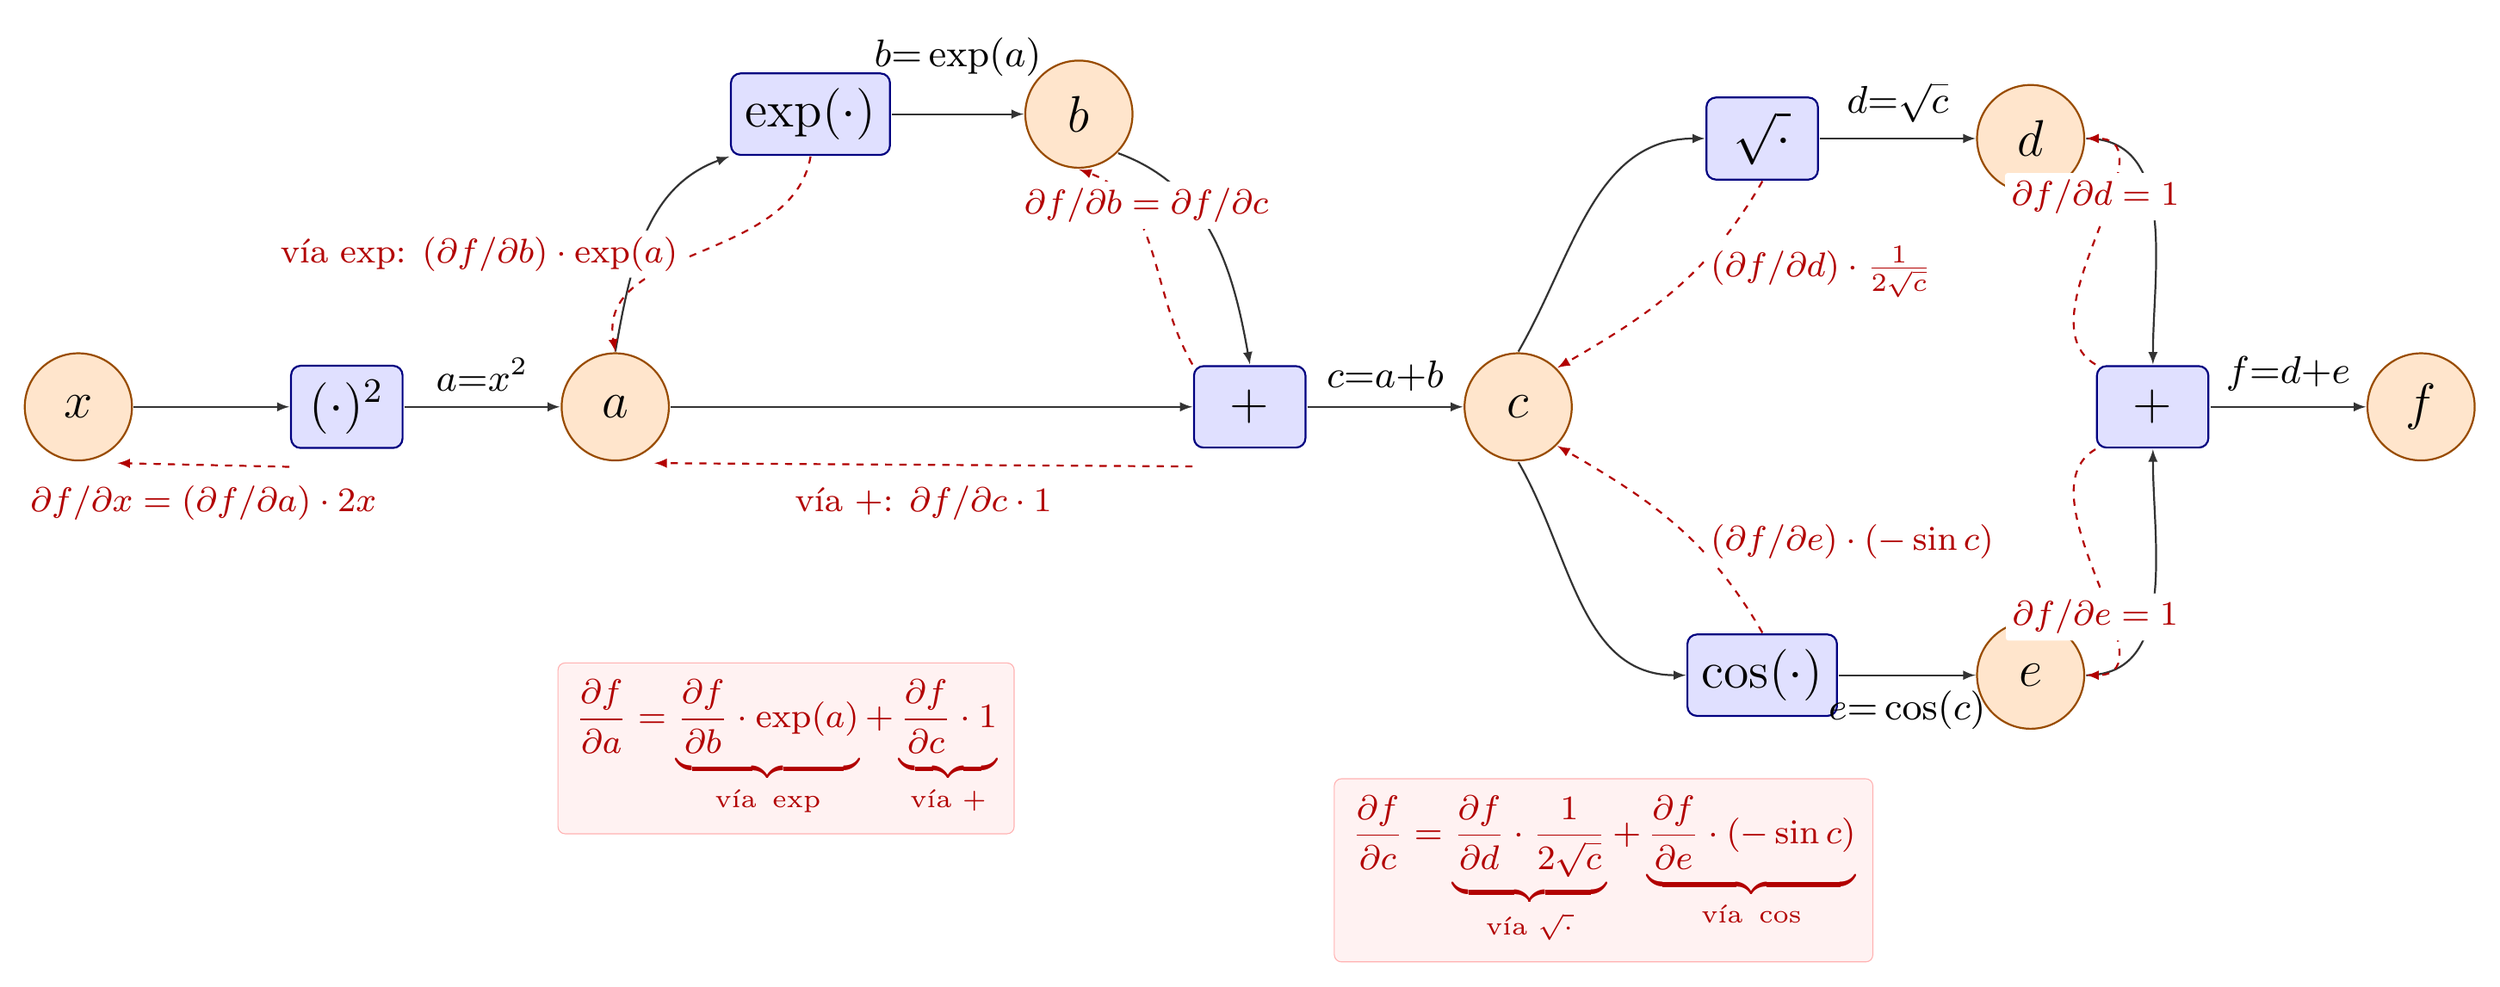
\begin{tikzpicture}[
    scale=1.8, transform shape,
    >=LaTeX,
    var/.style={
        circle,
        minimum width=2.5em,
        draw=orange!60!black,
        fill=orange!20,
        thick,
        font=\large
    },
    op/.style={
        rectangle,
        rounded corners=4pt,
        minimum width=2.6em,
        minimum height=1.9em,
        draw=blue!50!black,
        fill=blue!12,
        thick,
        font=\large
    },
    arrow/.style={-latex, thick, black!80},
    backprop/.style={-latex, dashed, red!70!black, thick},
    bplabel/.style={font=\footnotesize, text=red!70!black, fill=white,
                    inner sep=1.5pt, rounded corners=1pt},
    fwlabel/.style={font=\small, black}
]

% ══════════════════════════════════════════════════════════════════════════════
% NODOS — redistribuidos para equilibrio visual
% ══════════════════════════════════════════════════════════════════════════════

% Fila central
\node[var] (x)       at (0,      0)    {$x$};
\node[op]  (op_sq)   at (2.2,    0)    {$(\cdot)^2$};
\node[var] (a)       at (4.4,    0)    {$a$};
\node[op]  (op_add1) at (9.6,    0)    {$+$};
\node[var] (c)       at (11.8,   0)    {$c$};
\node[op]  (op_add2) at (17.0,   0)    {$+$};
\node[var] (f)       at (19.2,   0)    {$f$};

% Rama superior izquierda: exp y b — centrados entre a y +
\node[op]  (op_exp)  at (6.0,    2.4)  {$\exp(\cdot)$};
\node[var] (b)       at (8.2,    2.4)  {$b$};

% Rama superior derecha: sqrt y d
\node[op]  (op_sqrt) at (13.8,   2.2)  {$\sqrt{\cdot}$};
\node[var] (d)       at (16.0,   2.2)  {$d$};

% Rama inferior derecha: cos y e
\node[op]  (op_cos)  at (13.8,  -2.2)  {$\cos(\cdot)$};
\node[var] (e)       at (16.0,  -2.2)  {$e$};

% ══════════════════════════════════════════════════════════════════════════════
% FORWARD PASS — flechas sólidas con curvas suaves
% ══════════════════════════════════════════════════════════════════════════════

% x → (·)² → a
\draw[arrow] (x.east) -- (op_sq.west);
\draw[arrow] (op_sq.east) -- (a.west)
    node[midway, above, fwlabel] {$a{=}x^2$};

% a ↗ exp(·) → b  (curva suave hacia arriba)
\draw[arrow] (a.north) to[out=80, in=200] (op_exp.south west);
\draw[arrow] (op_exp.east) -- (b.west)
    node[midway, above, yshift=5pt, fwlabel] {$b{=}\exp(a)$};

% a → + (línea directa central)
\draw[arrow] (a.east) -- (op_add1.west);

% b ↘ + (curva suave bajando — simétrica a la subida de a→exp)
\draw[arrow] (b.south east) to[out=-20, in=100] (op_add1.north);

% + → c
\draw[arrow] (op_add1.east) -- (c.west)
    node[midway, above, fwlabel] {$c{=}a{+}b$};

% c ↗ √· → d  (curva simétrica hacia arriba)
\draw[arrow] (c.north) to[out=60, in=180] (op_sqrt.west);
\draw[arrow] (op_sqrt.east) -- (d.west)
    node[midway, above, fwlabel] {$d{=}\sqrt{c}$};

% c ↘ cos(·) → e  (curva simétrica hacia abajo)
\draw[arrow] (c.south) to[out=-60, in=180] (op_cos.west);
\draw[arrow] (op_cos.east) -- (e.west)
    node[midway, below, fwlabel] {$e{=}\cos(c)$};

% d ↘ +  (curva bajando — simétrica)
\draw[arrow] (d.east) to[out=0, in=90] (op_add2.north);

% e ↗ +  (curva subiendo — simétrica)
\draw[arrow] (e.east) to[out=0, in=-90] (op_add2.south);

% + → f
\draw[arrow] (op_add2.east) -- (f.west)
    node[midway, above, fwlabel] {$f{=}d{+}e$};

% ══════════════════════════════════════════════════════════════════════════════
% BACKPROPAGATION — flechas discontinuas rojas
% ══════════════════════════════════════════════════════════════════════════════

% [1] f → d : ∂f/∂d = 1
\draw[backprop] (op_add2.north west) to[out=150, in=0]
    node[bplabel, above=3pt, pos=0.5]
    {$\partial f / \partial d = 1$}
    (d.east);

% [2] f → e : ∂f/∂e = 1
\draw[backprop] (op_add2.south west) to[out=-150, in=0]
    node[bplabel, below=3pt, pos=0.5]
    {$\partial f / \partial e = 1$}
    (e.east);

% [3] d → c (vía √) : gradiente por rama superior
\draw[backprop] (op_sqrt.south) to[out=-120, in=30]
    node[bplabel, right=2pt, pos=0.4]
    {$(\partial f/\partial d)\cdot\frac{1}{2\sqrt{c}}$}
    (c.north east);

% [4] e → c (vía cos) : gradiente por rama inferior
\draw[backprop] (op_cos.north) to[out=120, in=-30]
    node[bplabel, right=2pt, pos=0.4]
    {$(\partial f/\partial e)\cdot(-\sin c)$}
    (c.south east);

% [5] + → b : ∂f/∂b = ∂f/∂c  (curva suave subiendo)
\draw[backprop] (op_add1.north west) to[out=120, in=-20]
    node[bplabel, above=2pt, pos=0.55]
    {$\partial f/\partial b = \partial f/\partial c$}
    (b.south);

% [6] + → a directo : contribución vía +
\draw[backprop] ([yshift=-4pt]op_add1.south west) -- ([yshift=-4pt]a.south east)
    node[bplabel, below=3pt, pos=0.5]
    {vía $+$: $\partial f/\partial c \cdot 1$};

% [7] exp → a : contribución vía exp  (curva suave bajando)
\draw[backprop] (op_exp.south) to[out=-100, in=100]
    node[bplabel, left=3pt, pos=0.5]
    {vía $\exp$: $(\partial f/\partial b)\cdot\exp(a)$}
    (a.north);

% [8] (·)² → x : ∂f/∂x
\draw[backprop] ([yshift=-4pt]op_sq.south west) -- ([yshift=-4pt]x.south east)
    node[bplabel, below=3pt, pos=0.5]
    {$\partial f/\partial x = (\partial f/\partial a)\cdot 2x$};

% ══════════════════════════════════════════════════════════════════════════════
% ANOTACIONES — cajas resumen de bifurcaciones
% ══════════════════════════════════════════════════════════════════════════════

% ∂f/∂a (bifurcación en a)
\node[font=\footnotesize, text=red!70!black, align=center,
      fill=red!5, draw=red!30, rounded corners=3pt, inner sep=4pt]
    at (5.8, -2.8)
    {$\displaystyle\frac{\partial f}{\partial a}
      = \underbrace{\frac{\partial f}{\partial b}\cdot\exp(a)}_{\text{vía }\exp}
      + \underbrace{\frac{\partial f}{\partial c}\cdot 1}_{\text{vía }+}$};

% ∂f/∂c (bifurcación en c)
\node[font=\footnotesize, text=red!70!black, align=center,
      fill=red!5, draw=red!30, rounded corners=3pt, inner sep=4pt]
    at (12.5, -3.8)
    {$\displaystyle\frac{\partial f}{\partial c}
      = \underbrace{\frac{\partial f}{\partial d}\cdot\frac{1}{2\sqrt{c}}}_{\text{vía }\sqrt{\cdot}}
      + \underbrace{\frac{\partial f}{\partial e}\cdot(-\sin c)}_{\text{vía }\cos}$};

\end{tikzpicture}
\end{document}
